%%This is a very basic article template.
%%There is just one section and two subsections.
\documentclass[11pt,twocolumn,varwidth=true,a4paper,fleqn]{article}
% \usepackage{fullpage}
% \usepackage{url}
% \usepackage[margin=1.1in]{geometry}
% \usepackage{graphicx}
% \usepackage{csvsimple}
% \usepackage{varwidth}
% \usepackage{array}
% \usepackage{float}
% \usepackage{pgfplotstable}
\usepackage[T1]{fontenc}
% \usepackage[compact]{titlesec}
% \usepackage{authblk}
\usepackage{bbm}

\usepackage{amsthm}
% \usepackage{amsmath}
\usepackage[utf8]{inputenc}
% \usepackage[english]{babel}
% \usepackage[nottoc]{tocbibind}
% %\usepackage[style=authoryear,backend=biber]{biblatex}
% \usepackage[backend=bibtex]{biblatex}
% \usepackage{biblatex}

\usepackage{graphicx}
\usepackage{csvsimple}
\usepackage{array}
\usepackage{float}
\usepackage{amsmath}
\usepackage{pgfplotstable}



\newtheorem{lemma}{Lemma}
\newtheorem{definition}{Definition}
\newtheorem{remark}{Remark}
\newtheorem{corollary}{Corollary}
 
\begin{document}
\nocite{*}

\title{Linear Discriminant Analysis Models of Distributed Streams}
\date{}
\maketitle

\begin{abstract}
Linear discriminant Analysis (LDA) is widely used calssificatio and
dimensionality reduction in many fields.
As data evolves, LDA models must be recomputed. 
In distributed streaming settings, however, periodically recomputing the global model is
wasteful: communicating new observations or model updates
is required even when the model is, in practice, unchanged.
This is prohibitive in many settings, such as in wireless sensor
networks, or when the number of nodes is very large. The
alternative, monitoring prediction accuracy, is not always
sufficient: in some settings, for example, we are interested in
the model's coefficients, rather than its predictions.
We propose the first monitoring algorithm for LDA models of distributed data
streams that guarantees a bounded model error. It maintains an accurate estimate
using a fraction of the communication by recomputing only
when the precomputed model is suffiengly far from the
(hypothetical) current global model. When the global model
is stable, no communication is needed.
Experiments on real and synthetic datasets show that
our approach reduces communication by up to two orders
of magnitude while providing an accurate estimate of the
current global model in all nodes.
\end{abstract}

\section{Introduction}
\par Fisher's linear discriminant \cite{fisher1936use}, a method used in statistics, 
pattern recognition and machine learning to find a linear combination of features 
that characterizes or separates two or more classes of objects or events. 
The resulting combination may be used as a linear classifier, or, 
more commonly, for dimensionality reduction before later classification.
\\\par FLD approaches the problem by assuming that the conditional probability density functions $P(\vec x|y=p)$ and $P(\vec x|y=q)$ are both normally distributed with mean and covariance parameters $\left(\vec \mu_p, B_p\right)$ and $\left(\vec \mu_q, B_q\right)$, for two target classes p and q respectively.
%\\$w \propto (S_p+S_q)^{-1}(\mu_p - \mu_q)$
\\Under this assumption, the Bayes optimal decision criterion is a threshold on the dot product
\begin{equation*} \label{eq:decision}
w \cdot x > c
\end{equation*}
for some threshold constant c, where
\begin{equation} \label{eq:w}
w \propto (B_p+B_q)^{-1}(\mu_p - \mu_q)
\end{equation}
\begin{equation} \label{eq:c}
c = \frac{1}{2}(T-{\mu_p}^T S_p^{-1} {\mu_p}+{\mu_q}^T S_q^{-1} {\mu_q})
\end{equation}
\subsection{Our Contribution}

\begin{figure}[h]
\centering
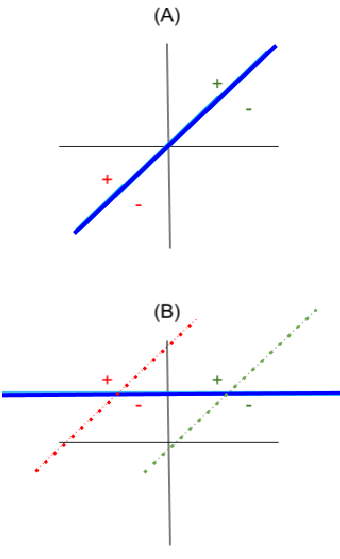
\includegraphics[width=60mm]{NegativeExample.png}
\caption{Example of false monitoring by applying the local LDA formula. The
initial state of the data is presented in (A) and the state in a later point
is shown in (B). In (B) every node (green and red) calculates the same angle
for the separtor  as it was in (A), i.e., no violation is made. But it can be
seen the true separtor (blue dashed line) angle is significantly changed.}
\label{NegativeExampl}

\end{figure}
\section{Related Work}
\subsection{Distributed Monitoring}
The last decade witnessed a sharp increase in work on imposing local conditions for monitoring the value of a function
defined over distributed nodes. While the general problem is NP-complete
\cite{keren2014geometric}, considerable progress has been made for real-life problems. Most work dealt with the simpler cases of
linear functions \cite{keralapura2006communication, kashyap2008efficient}, as well as monotonic
functions \cite{michel2005klee}.
Some papers addressed non-linear problems, e.g., monitoring
the value of a single-variable polynomial \cite{shah2008handling}, and analysis
of eigenvalue perturbation \cite{huang2007communication}. 
In \cite{sharfman2007geometric} a geometric approach for monitoring arbitrary functions over distributed
streams was proposed, and later extended and generalized
\cite{keren2012shape,lazerson2015monitoring}. However, nearly all work on geometric monitoring addressed
functions which are either polynomials (typically quadratic), or defined by
compositions of polynomial with simple functions such as medians and quotients. 
The closest work to ours is on Least Square Regression
\cite{gabel2015monitoring}, we will harness some of their mathematical lemmas
for our LDA problem. To the best of our knowledge, the problem addressed in this
paper monitoring the LDA model was never addressed over a distributed setting. Note
that the monitored function contains the highly complicated
operation of matrix inversion, which is not linear or convex,
and which, when written explicitly, becomes intractable even
for relatively low dimensions (e.g., the analytic expression
for the inverse of a $20 \times 20$ matrix involves polynomials with
$20!$ monomials). Therefore, a straightforward application of
previous work on geometric monitoring is impossible.

\section{Problem Definition}
\subsection{Monitoring LDA of Distributed Streams}
Assume that the observations ${(x^i_j; y^i_j)}$ are distributed across k nodes, and that these observations are dynamic (they change over time, as nodes receive new observations that replace older ones. As data evolves, it is possible that the
previously computed model no longer matches the current true model. We wish to maintain an accurate estimation $w_0$ of the current global FLD model, $w$. The question is then when to update the model.

Let $w_0$ be the existing model (vector of weights of a linear classifier), 
previously computed at some point in the past (the synchronization time), 
and let $w$ be the true (if we had aggregated the current observations 
from all of the nodes into one place and computed the model according to it) FLD model. 
Given an error threshold $T$, our goal is to raise an alert if
\begin{equation} \label{eq:coneCritiria}
\frac{<w,w_0>}{\parallel w \parallel \parallel w_0 \parallel}  < T
\end{equation}
\\We will monitor the maximal voluem sphere around $w_0$ that resides completely
inside the cone from equation~\ref{eq:coneCritiria}. This sphere is
defined by
\begin{equation} \label{eq:critiria}
\parallel w-w_0 \parallel \  >  R_0
\end{equation}
Where $R_0 := \  \parallel w_0 \parallel \sqrt{1-T^2}$ is the maximal radius.
\section{Monitoring Distributed LDA With Convex Subsets}
\subsection{Notation}
$k$ - number of nodes
\\$n$ - number of vectors in a node
\\$x^i_j$ - the j'th vector in the i'th node
\\$y^i_j$ - the label (p or q) of $x^i_j$
%\\ D - sample of $n \cdot k$ labeled observations ${(x^i_j, y^i_j)}$
\\$N_p$  - total number of observations from class P, from all of the nodes
\\$N_q$  - total number of observations from class Q, from all of the nodes
\\$N_p^i$  - total number of observations from class P, in the i'th node
\\$N_q^i$  - total number of observations from class Q, in the i'th node
\\
\\$p,q,p^i$ and $q^i$  are the global and local mean of the classes,
i.e.:
\\$p^i := \frac{1}{N_p^i}\sum_{j=1}^{n}\mathbbm{1}{(y^i_j=P)}x^i_j
\\q^i := \frac{1}{N_q^i}\sum_{j=1}^{n}\mathbbm{1}{(y^i_j=Q)}x^i_j
\\p := \frac{1}{N_p}
\sum_{i=1}^k\sum_{j=1}^n\mathbbm{1}{(y^i_j=P)}x^i_j=\frac{1}{k}\sum_{i=1}^kp^i 
\\q:=\frac{1}{N_q} \sum_{i=1}^k\sum_{j=1}^n\mathbbm{1}{(y^i_j=Q)}x^i_j =
\frac{1}{k}\sum_{i=1}^kq^i$
\\
\\$S$ and $S^i$  are the global and local normalized scatter matrices:
\\$S^i := \frac{1}{n}\sum_{j=1}^{n}x^i_j(x^i_j)^T
\\S := \frac{1}{nk}
\sum_{i=1}^k\sum_{j=1}^nx^i_j(x^i_j)^T=\frac{1}{k}\sum_{i=1}^kS^i$
\\Simillarly, $u$ and $u^i$ are the distance between the classes centroids
\\$u:=p - q$
\\$u^i:=p^i - qi$
\\ $B$ is the global covariance matrix:
\\$B:=S - pp^T - qq^T$
%\\B^i:=S^i - p^i(p^i)^T - q^i(q^i)^T$
\\\\Let w be our current true model, following Eq.~\ref{eq:w}, we can denote:
%\\$w(S,\mu_p,\mu_q) := (S - \mu_p\mu_p^T - \mu_q\mu_q^T)^{-1}(\mu_p - \mu_q)$
\begin{equation*}
w:=(S - pp^T - qq^T)^{-1}(p-q)=B^{-1}u
\end{equation*}
Let $w_0$ be the existing model, previously computed from $S_0, p_0$ and $q_0$
or from $B_0$ and $u_0$ at some point in the past (the synchronization time),
then
\begin{equation*} 
w_0:=(S_0 - p_0p_0^T - q_0q_0^T)^{-1}(p_0-q_0)=B_0^{-1}u_0
\end{equation*}
$\Delta_s, \delta_p$, and $\delta_q$ are the drift vectors of $S, p$, and $q$, i.e.:
$
\\\Delta_s:= S - S_0
\\\delta_p:= p - p_0
\\\delta_q := q - q_0$
\\If $S_0^i$, $p_0^i$ and $q_0^i$ are the local normalized scatter and averages
of the samples in a node, we can define the local drift to be:
$
\\\Delta_s^i:= S^i - S_0^i
\\\delta_p^i:= p^i - p_0^i
\\\delta_q^i:= q^i - q_0^i
$
\begin{remark} \label{average}
It easy to notice that every global drift is the average of the local drifts:
\begin{equation*}
\Delta_s = \frac{1}{k} \sum \Delta_s^i, \\
\delta_p = \frac{1}{k} \sum \delta_p^i, \\
\delta_q = \frac{1}{k} \sum \delta_q^i 
\end{equation*}
\end{remark}

\subsection{Convex Safe Zones}
We propose to solve the monitoring problem by means of
``good'' convex subsets, called safe zones, of the data space.
Each node monitors its own drift: as long as current values
at local nodes $(S^i,p^i,q^i)$ are sufficiently similar to their values
at sync time $(S^i_0,p^i_0,q^i_0))$, $w_0$ is guaranteed to be close to $w$.
Formally, we define a convex subset $\mathcal{C}$ such that:
\begin{equation} \label{convex}
(\Delta_s, \delta_p, \delta_q) \in \mathcal{C} \Rightarrow \parallel w-w_0
\parallel \ < R_0
\end{equation}
\begin{lemma}
Let $\mathcal{C}$ be a convex subset that satisfies Eq. \ref{convex}.
If $(\Delta_s^i, \delta_p^i, \delta_q^i) \in \mathcal{C}$ for all i, then
\begin{equation*}
\parallel w-w_0 \parallel \ < R_0
\end{equation*}
\end{lemma}
\begin{proof}
Express $S, p$ and $q$ as their values at synchronization with the addition of the
average of the local drifts:
\begin{equation*} 
\begin{split}
(S,p,q) & = \frac{1}{k} \sum_i (S^i,p^i,p^j) \\
 & = (S_0,p_0,q_0) + \frac{1}{k} \sum_i (\Delta_s^i,\delta^i_p,\delta_q^i) \\
\end{split}
\end{equation*}
From $\mathcal{C}$'s convexity and using Remark \ref{average} we get:
\begin{equation*} 
\begin{split}
\forall i (\Delta_s^i,\delta^i_p,\delta_q^i) \in \mathcal{C} & \Rightarrow 
\frac{1}{k} \sum_i (\Delta_s^i,\delta^i_p,\delta_q^i) \in \mathcal{C} \\
& \Rightarrow (\Delta_s,\delta_p,\delta_q) \in \mathcal{C}
\end{split}
\end{equation*}
Finally, from the definition of $\mathcal{C}$ we obtain:
\begin{equation*}
(\Delta_s,\delta_p,\delta_q) \in \mathcal{C} \Rightarrow \parallel w-w_0
\parallel \ < R_0
\end{equation*}
which completes the proof.
\end{proof}

\subsection{Sliding Window Convex Bound}
In the sliding window model each node computes $S^i$ from the $L$ samples seen
at node $i$, while $S_0^i$ (and hence $S_0$) is built from the last L samples before
sync. 
We denote the drift in the global covariance matrix
\begin{alignat*}{2}
\Delta & := && B-B_0 \\
& = && (S_0+\Delta_S - (p_0+\delta_p)(p_0+\delta_p)^T \\
& && - (q_0+\delta_q)(q_0+\delta_q)^T) \\
& && - (S_0 - p_0p_0^T - q_0q_0^T) \\
& = && - \delta_p\delta_p^T - \delta_q\delta_q^T \\
& && + \Delta_S - p_0\delta_p^T \\
& && - \delta_pp_0^T - q_0\delta_q^T - \delta_qq_0^T
\end{alignat*}
we break $\Delta$ into its quadratic part
\begin{equation*}
M:= - \delta_p\delta_p^T - \delta_q\delta_q^T, 
\end{equation*}
and linear part
\begin{equation*}
L:= \Delta_S - p_0\delta_p^T - \delta_pp_0^T - q_0\delta_q^T - \delta_qq_0^T, 
\end{equation*}
and hence 
\begin{equation*}
\Delta= L+ M.
\end{equation*}
We denote the drift of the distance between the centroids:
\begin{equation*}
\delta:= u-u_0 = \delta_p - \delta_q
\end{equation*}
Now we can state a convex bound for our problem is:
\begin{lemma} \label{convexBound}
If $\mathcal{G}$ is the set of triplets $(\Delta_s^i, \delta_p^i, \delta_q^i)$
 that satisfies the bound:
 \begin{equation*} 
\begin{split}
||B_0^{-1}\delta|| &+ (||w_0||+R_0)(||B_0^{-1}L||+||B_0^{-1}M||) \\ & \leq  R_0
\end{split}
\end{equation*}
and satisfies the inequality:
 \begin{equation*} 
||B_0^{-1}\Delta|| < 1
\end{equation*}
 then $\mathcal{G}
 \subseteq \mathcal{C}$ and $\mathcal{G}$ is convex.
Where $||A||$ is the operator norm of the matrix A.
\end{lemma}
The proof of the lemma \ref{convexBound} quite technical, and
the details are available in Appendix A.

\subsection{Probabilistic Distributed LDA Monitoring}
In this section we will develop a probabistic framwork for violation recopvery.
We call it Probabilistic Distributed LDA Monitoring (PLDA). The basic idea is
not to sync when a single node is violated but when the vilations amount is
above a certin threshold. The derivation of this threshold is shown below:

Let $TV \in {0,1}$ stand for the indicator for True
Violation, then  
\begin{equation*}
P_{TV} := P(TV = 1),
\end{equation*}
and let $v_i \in {0,1}$ stand for the indicator for a local violation in the
i'th node. The probability for True Positive (TP) and False Positive (FP) in a
node is:
\begin{alignat*}{1}
& P_{TP} := P(v_i=1 | TV=1) \\
& P_{FP} := P(v_i=1 | TV=0)
\end{alignat*}
Let $V$ be the random variable of the number of local violations
\begin{equation*}
V := \sum_{i=1}^k v_i,
\end{equation*}
\begin{alignat*}{1}
& B_{TP} := P(V=v | TV=1) \propto Bin(k,P_{TP}) \\
& B_{FP} := P(V=v | TV=0) \propto Bin(k,P_{TF})
\end{alignat*}
We would like to monitor the probability for TV, i.e. $P(TV=1|V=v)$. Using
Bayes' rule we can derive
\begin{alignat*}{1}
& P(TV=1|V=v) \\
& = \frac{P(V=v, TV=1)}{P(V=v)}\\
& = \frac{P(V=v|TV=1)P(TV=1)}{P(V=v)} \\
& = \frac{P_{TV}B_{TP}}{P_{TV}B_{TP} + (1-P_{TV})B_{FP}}
\end{alignat*}

If we assume $P_{TP}=1$, it is simplfied to:
\begin{equation*}
P(TV=1|V=v) = \frac{B_{TP}}{P_{TV}B_{TP} + (1-P_{TV})B_{FP}}
\end{equation*}
\section{Evaluation}
\subsection{Synthetic Datasets}

\subsubsection{Effect of Threshold}
Is seen in Fig \ref{PERvsDLDAoverTime} and in Fig  \ref{PERvsDLDAoverError}.
	\begin{figure*}[ht]
	\centering
	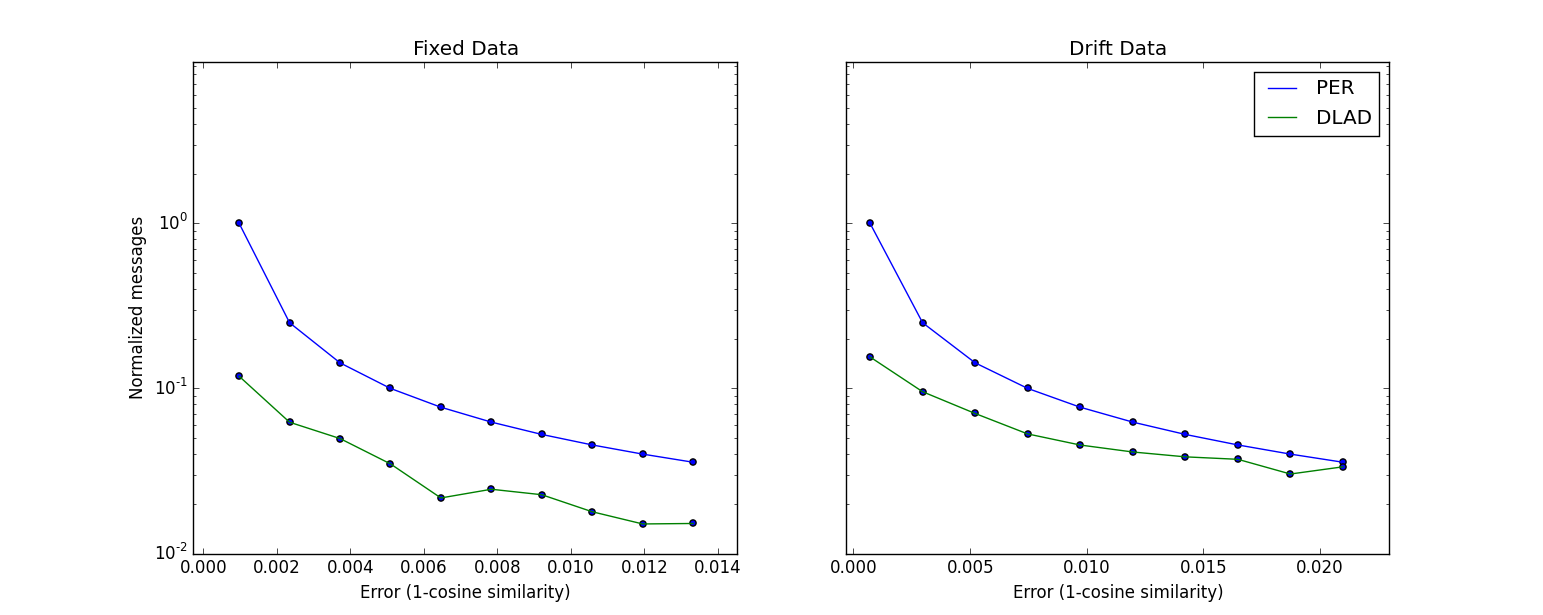
\includegraphics[width=\textwidth]{PER/PERvsDLDAoverError.png}
	\caption{One node naive sync.png}
	\label{PERvsDLDAoverError}
	\end{figure*}

	\begin{figure*}[ht]
	\centering
	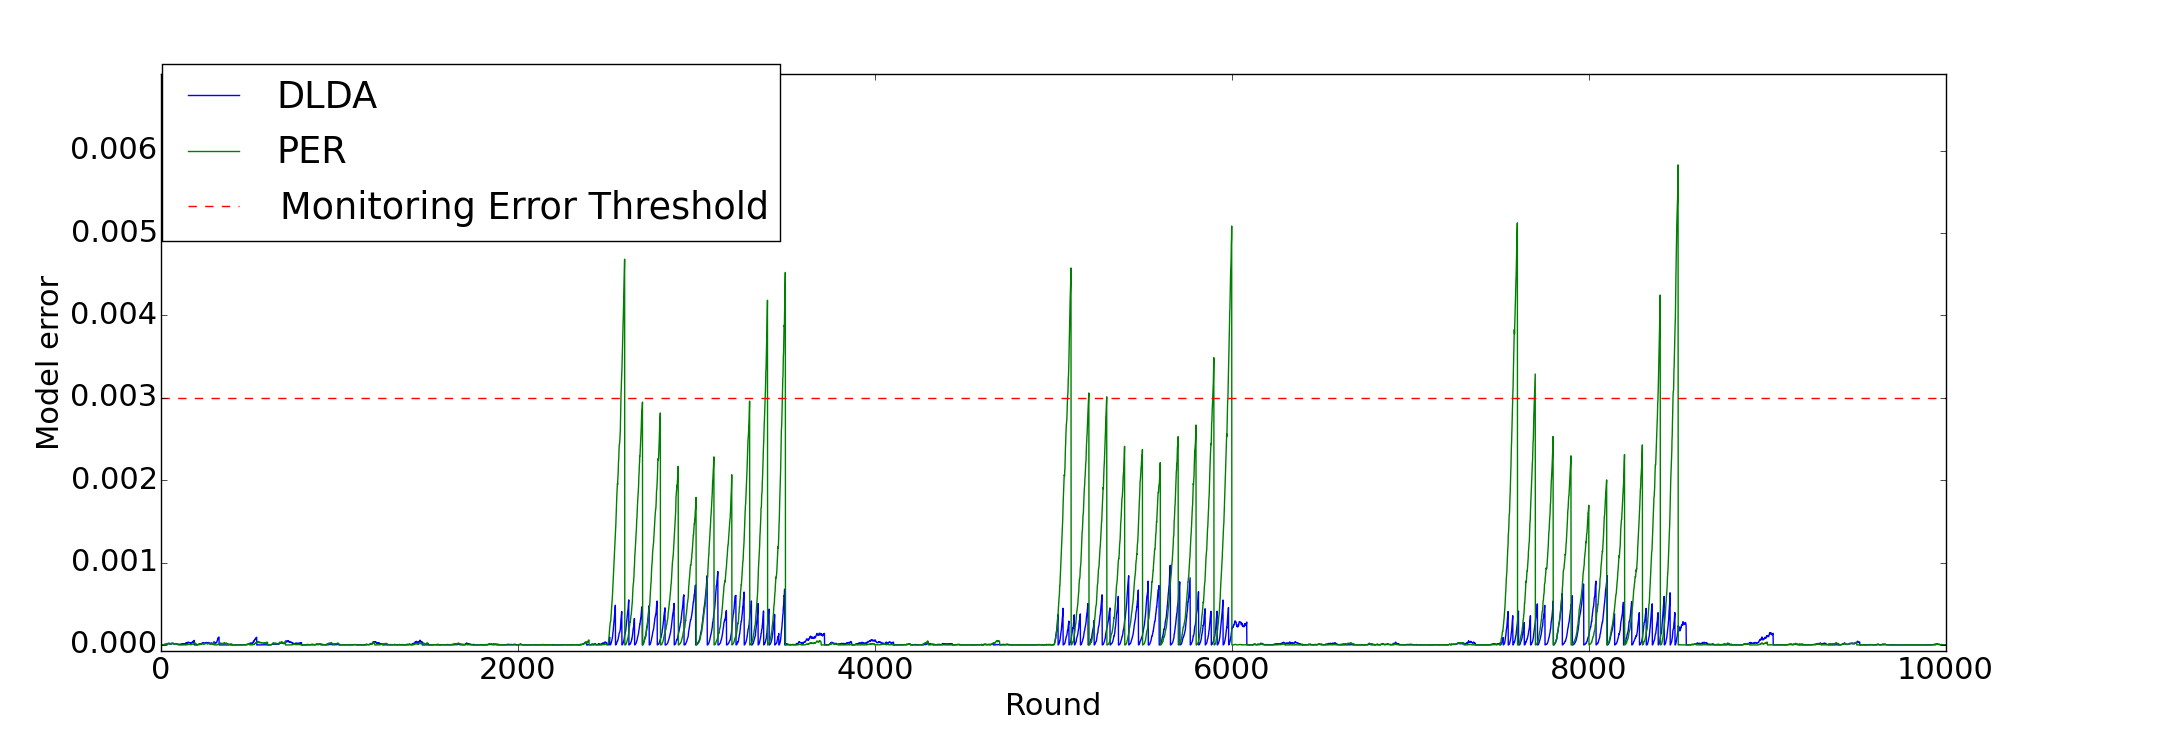
\includegraphics[width=\textwidth]{PER/PERvsDLDAoverTime.png}
	\caption{One node naive sync.png}
	\label{PERvsDLDAoverTime}
	\end{figure*}
\subsubsection{Scalability}
Is seen in Fig \ref{Nodes}.
	\begin{figure}[h]
	\centering
	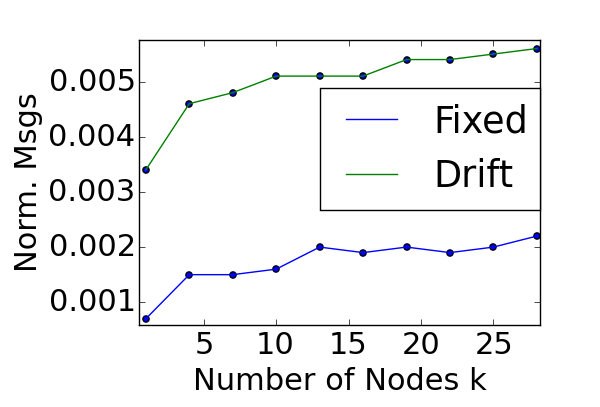
\includegraphics[width=60mm]{CommunicationOfFixedVsDrift/Nodes.png}
	\caption{Communication As Function Of the amount of nodes}
	\label{Nodes}
	\end{figure}
\subsubsection{Dimension}
Is seen in Fig \ref{Dimension}.
	\begin{figure}[h]
	\centering
	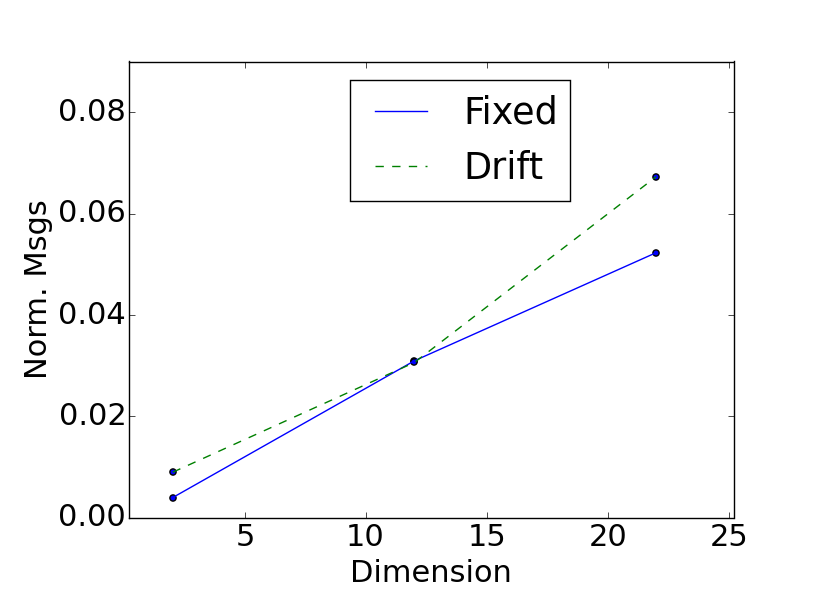
\includegraphics[width=60mm]{CommunicationOfFixedVsDrift/Dimension.png}
	\caption{Communication As Function Of the input's dimension}
	\label{Dimension}
	\end{figure}
\subsubsection{Window Size}
Is seen in Fig \ref{WindowSize}.
	\begin{figure}[h]
	\centering
	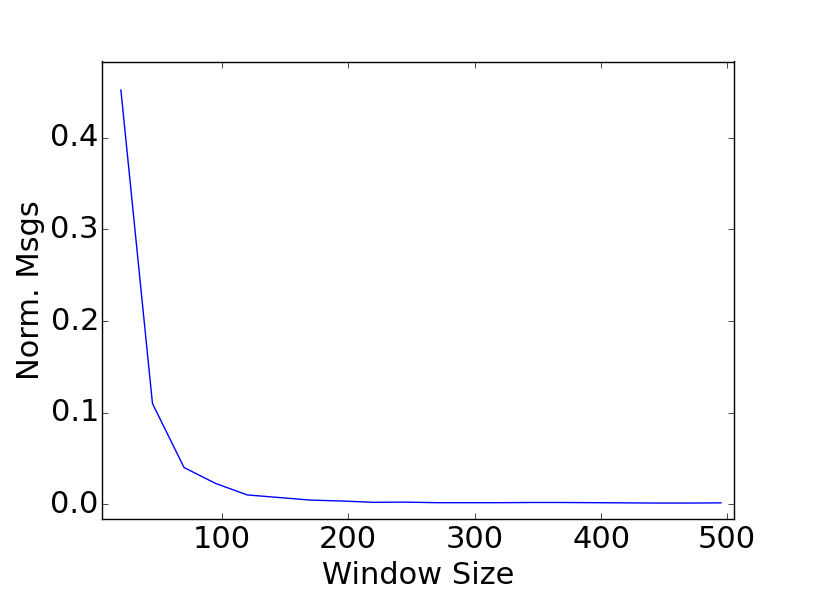
\includegraphics[width=60mm]{CommunicationOfFixedVsDrift/WindowSize.png}
	\caption{Communication As Function Of Window Size}
	\label{WindowSize}
	\end{figure}
\subsubsection{Noise}
Is seen in Fig \ref{Noise}.
	\begin{figure}[h]
	\centering
	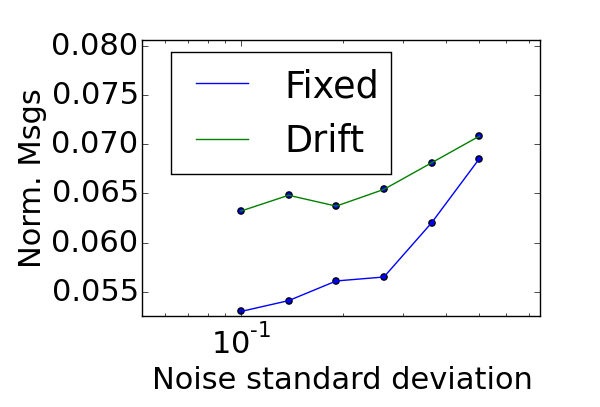
\includegraphics[width=60mm]{CommunicationOfFixedVsDrift/Noise.png}
	\caption{Communication As Function Of standard deviation of the Gaussians that
	generates the data}
	\label{Noise}
	\end{figure}

\section{Real Data Experiments}
In this section we will demonstrate the algorithm with 3 datasest. The first
(New Messages Users Preference Monitoring) is relativly small, and a small scale
scenario will be demonstarated on it using the deterministic DLDA. 
\subsection{New Messages Users Preference Monitoring}
\cite{usenet}
\subsection{Power Consumtion Monitoring}
The dataset contains hourly power supply of an Italy electricity company which
records the power from two sources: power supply from main grid and power 
transformed from other grids. This stream contains three year power supply records 
from 1995 to 1998, and our learning task is to predict which hour (1 out of 24 hours) the 
current power supply belongs to. The concept drifting in this stream is mainly 
driven by the issues such as the season, weather, hours of a day (e.g., morning 
and evening), and the differences between working days and weekend.  
This dataset is described and can be downloaded in \cite{powerSupply}.
The binary classifcation that was chosen for the demonstration is given a power
supply measurment, decide if it is a night or a day. This is an
example for gradual concept drift adaptation (seasons do not change suddenly).


\begin{figure*}[h]
\centering
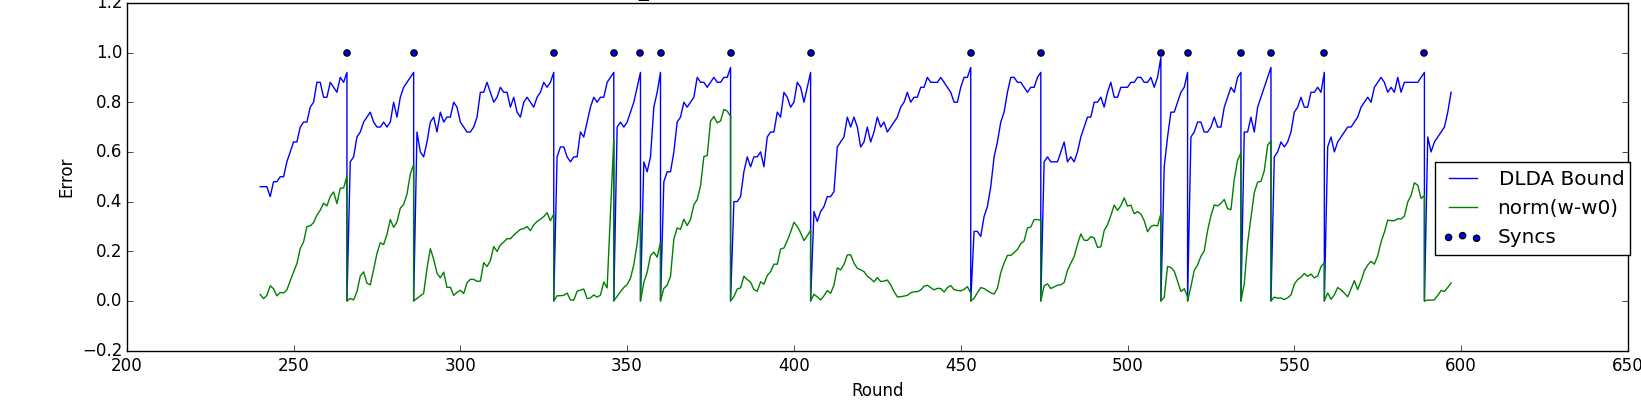
\includegraphics[width=\textwidth]{PowerSupply/errorComparison.png}
\caption{An adaptation to a gradual concept drift of the power
supply dataset is demonstrated by a comparison between the fraction (out of 50)
of violated according to the local DLDA bound nodes (blue), to the true error in the 
norm of the whole data aggregated from all of the nodes (green).}
\label{PowerSupply}
\end{figure*}

\subsection{Gas Sensor Time Series Monitoring}
Data in this experiment consists of measurements collected
by an array of 16 chemical sensors recorded at a sampling
rate of 100Hz for 24 hours, resulting in 8378504 data points for each sensor. 
This dataset is described in \cite{bigGas}.
At the first 12 hours the task is to obtain the exsitence of Carbon monoxide
(CO) and from the 13'th hour the task is to obtain the exsitence of Methane. The
change between the first task and the second is the CD that should be
detected. In Fig \ref{BigGasShowData} a PCA projection of the data is shown.

\begin{figure}[h]
\centering
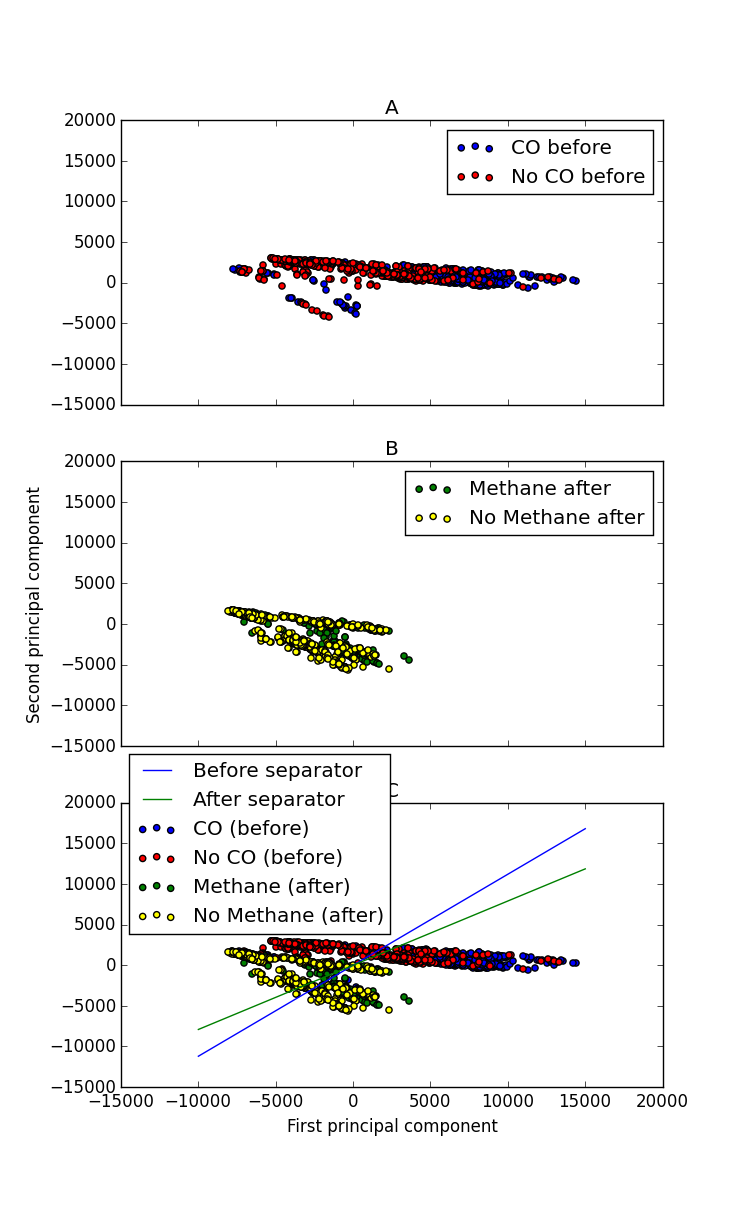
\includegraphics[width=60mm]{BigGas/showData.png}
\caption{2 dimension PCA projection of the data, before the CD (A),
after the CD (B), and all of the data together with the LDA separator of each
period (C). It can be seen that there is a differnce in the separator's
direction between the periods.}
\label{BigGasShowData}
\end{figure}

\bibliographystyle{unsrt}
\bibliography{bib}


\clearpage
\appendix
\section{Appendix} \label{AppendixA}
To find a convex subset C satisfying the condition of Eq. \ref{convex}. 
First we define operator norm:
\begin{definition}
Let $A$ be a matrix. Its operator norm, or
spectral norm, hereafter just norm, is defined as:
\begin{equation*}
||A|| = \sup_{x \neq 0}\frac{||Ax||}{||x||} 
\end{equation*}
\end{definition}

\begin{lemma} \label{lemma:newman}
If A is square and $||A|| < 1$, then
\begin{equation*}
||(I+A)^{-1}|| < \frac{1}{1-||A||}
\end{equation*}
\end{lemma}
The proof for this lemma can be found in Gabel's paper
\cite{gabel2015monitoring}.

\subsection{Convex Bound Proof}
\begin{lemma}
$\mathcal{G} \subseteq \mathcal{C}$:
\end{lemma}

\begin{proof}
We can write the sphere condition in terms of $B_0, \Delta, u_0$ and $\delta$ using the triangle
inequality:
\begin{equation} \label{in}
\begin{split}
||w-w_0|| & = \ ||(B_0+\Delta)^{-1}(u_0+\delta) - B_0^{-1}u_0|| \\
& < ||(B_0+\Delta)^{-1}\delta|| \\
& \ \ + ||((B_0+\Delta)^{-1} - B_0^{-1})u_0||
\end{split}
\end{equation}

We split the last addition into two parts:
\begin{equation}  \label{e1e2}
\begin{split}
& E_1:= ||(B_0+\Delta)^{-1}\delta|| \\
& E_2:= ||((B_0+\Delta)^{-1} - B_0^{-1})u_0||
\end{split}
\end{equation}
If we assume that $||B_0^{-1}\Delta||\ \leq \ 1$, 
then from lemma \ref{lemma:newman} we get:
\begin{equation} \label{e1e2In}
\begin{split}
& E_1 \leq \frac{||B_0^{-1}\delta||}{1-||B_0^{-1}\Delta||} \\
& E_2 \leq  \frac{|| B_0^{-1}\Delta w_0||}{1-||B_0^{-1}\Delta||}
\end{split}
\end{equation}
From Cauchy-Schwarz inequality we get:
\begin{equation} \label{CS}
||B_0^{-1}\Delta w_0|| \ \leq \ ||B_0^{-1}\Delta||||w_0||
\end{equation}
Substitute Eq. \ref{e1e2}, \ref{e1e2In} and \ref{CS} in Eq. \ref{in}, and we
get:
\begin{equation}
\begin{split}
|| w-w_0 \parallel & \leq \ E_1+E_2 \\
& \leq \frac{||B_0^{-1}\delta|| + ||B_0^{-1}\Delta||||w_0||}{1 -||B_0^{-1}\Delta||} \\
& \leq R_0
\end{split}
\end{equation}
Losing the denominator:
\begin{equation} \label{lostDenom}
||B_0^{-1}\delta|| + ||B_0^{-1}\Delta||||w_0||
\leq R_0(1 -||B_0^{-1}\Delta||)
\end{equation}
From the triangle inequality we can rewrite:
\begin{equation} \label{linQuad}
||B_0^{-1}\Delta|| \leq ||B_0^{-1}L||+||B_0^{-1}M||
\end{equation}
And finally, from combining inequalities \ref{lostDenom} and \ref{linQuad},
we get the bound:
\begin{equation} \label{convexBound}
\begin{split}
||B_0^{-1}\delta|| &+ (||w_0||+R_0)(||B_0^{-1}L||+||B_0^{-1}M||) \\ & \leq  R_0
\end{split}
\end{equation}
\end{proof}

\begin{lemma} \label{delta}
$||B_0^{-1}\delta||$ is convex in $\delta$
\end{lemma}
\begin{proof}
By convexity definition, for a scalar $0 \leq \alpha \leq 1$: 
\begin{equation} 
\begin{split}
& ||B_0^{-1}(\alpha\delta_1+(1-\alpha)\delta_2)|| \\
= & ||\alpha B_0^{-1}\delta_1+(1-\alpha)B_0^{-1}\delta_2)|| \\
\leq & \alpha||B_0^{-1}\delta_1||+(1-\alpha)||B_0^{-1}\delta_2||
\end{split}
\end{equation}
Where the last inequality comes from the triangle inequality.
\end{proof}

We recall that:
\begin{equation*} 
L:= \Delta_S - p_0\delta_p^T - \delta_pp_0^T - q_0\delta_q^T - \delta_qq_0^T
\end{equation*}
\begin{lemma} \label{L}
$||B_0^{-1}L||$ is convex in $\Delta_s, \delta_p$
and $\delta_q$.
\end{lemma}
\begin{proof}
We show it from the definition of $L$ and convexity:
\begin{alignat*} {2}
& && ||\alpha\Delta_{s1}+(1-\alpha)\Delta_{s2} \\
& && - p_0(\alpha\delta_{p1}+(1-\alpha)\delta_{p2})^T \\
& && - (\alpha\delta_{p1}+(1-\alpha)\delta_{p2})p_0^T \\
& && - q_0(\alpha\delta_{q1}+(1-\alpha)\delta_{q2})^T \\
& && - (\alpha\delta_{q1}+(1-\alpha)\delta_{q2})q_0^T || \\
& = && ||\alpha(\Delta_{s1} - p_0\delta_{p1}^T - \delta_{p1}p_0^T \\
& && - q_0\delta_{q1}^T - \delta_{q1}q_0^T) \\
& && + (1-\alpha)\Delta_{s2} - p_0\delta_{p2}^T - \delta_{p2}p_0^T \\
& && - q_0\delta_{q2}^T - \delta_{q2}q_0^T)|| \\
& \leq && \alpha||\Delta_{s1} - p_0\delta_{p1}^T - \delta_{p1}p_0^T \\
& && - q_0\delta_{q1}^T - \delta_{q1}q_0^T|| \\
& && + (1-\alpha)||\Delta_{s2} - p_0\delta_{p2}^T - \delta_{p2}p_0^T \\
& && - q_0\delta_{q2}^T - \delta_{q2}q_0^T||
\end{alignat*}
\end{proof}

We recall that:
\begin{equation*} 
M:= - \delta_p\delta_p^T - \delta_q\delta_q^T
\end{equation*}
\begin{lemma} \label{M}
$||B_0^{-1}M||$ is convex in $\delta_p$
and $\delta_q$.
\end{lemma}
\begin{proof}
From the definition of operator norm, we can rewrite the function as:
\begin{alignat*} {2}
||M|| & = && \max_{||u||=1}{\{u^T \delta_p\delta_p^T u\}} + \max_{||u||=1}{\{u^T \delta_q\delta_q^T u\}} \\
& = && \max_{||u||=1}{\{||u^T \delta_p||^2\}} + \max_{||u||=1}{\{||u^T
\delta_q||^2\}}
\end{alignat*}
Noticing that max over a fininte number of convex function is also a convex
function end our proof.
\end{proof}

\begin{corollary}
From lemmas \ref{delta}, \ref{L} and \ref{M} we can conclud that $\mathcal{G}$
is convex.
\end{corollary}

\end{document}
